	\documentclass[12pt]{report}

\usepackage{amsmath,amsthm,amssymb,latexsym,amscd}
\usepackage{setspace, thesis}
\usepackage{caption}
%\usepackage[english]{babel}   % does not work with amsart
\usepackage{color}
\usepackage{dcolumn}
\usepackage{float}
\usepackage{graphicx}
\usepackage[latin9]{inputenc}
\usepackage{multirow}
\usepackage{rotating}
%\usepackage{subfigure}
\usepackage{wrapfig}
\usepackage{psfrag}
\usepackage{booktabs}
\usepackage{xspace}
\usepackage{tabularx}
\usepackage{tocloft}
\usepackage[hyphens]{url}
\usepackage{array}
\usepackage{listings}
\usepackage{framed}
%\usepackage[latin9]{inputenc}
%\usepackage{mathpazo}
\usepackage[hyphens]{url}

% Put this package last
\usepackage[pdftex,bookmarks=true,pdfborder=false,bookmarksopen,bookmarksnumbered]{hyperref}
% Put this package after hyperref
\usepackage[all]{hypcap}
\usepackage[nottoc]{tocbibind}
% Don't use tt font for urls
\urlstyle{rm}
\usepackage{comment}
\usepackage{paralist}

%\usepackage[margin=1in,nohead,foot=0.3in]{geometry}
\usepackage[margin=0.7in,nohead,foot=0.3in]{geometry}
%\usepackage[left=0.9in, right=0.9in, top=0.9in, bottom=0.7in]{geometry}

\newcommand{\todo}[1]{{\color{red}~\textsf{[#1]}}}
\newcommand{\up}{\vspace*{-1em}}
\newcommand{\upp}{\vspace*{-0.5em}}


\newcommand{\pilot}{Pilot\xspace}
\newcommand{\pilots}{Pilots\xspace}
\newcommand{\pilotjob}{Pilot-Job\xspace}
\newcommand{\pilotjobs}{Pilot-Jobs\xspace}
\newcommand{\pilotmapreduce}{Pilot-MapReduce\xspace}
\newcommand{\computeunit}{Compute Unit\xspace}
\newcommand{\computeunits}{Compute Units\xspace}
\newcommand{\cu}{CU\xspace}
\newcommand{\cus}{CUs\xspace}
\newcommand{\mrmg}{MR-Manager\xspace}
\newcommand{\cs}{Compute Service\xspace}
\newcommand{\css}{Compute Services\xspace}
\newcommand{\pcs}{Pilot Compute Service\xspace}
\newcommand{\dataunit}{Data Unit\xspace}
\newcommand{\dataunits}{Data Unit\xspace}
\newcommand{\du}{DU\xspace}
\newcommand{\dus}{DUs\xspace}
\newcommand{\pilotdata}{Pilot-Data\xspace}
\newcommand{\pd}{PD\xspace}
\newcommand{\pds}{Pilot Data Service\xspace}
\newcommand{\pdss}{Pilot Data Services\xspace}
\newcommand{\su}{SU\xspace}
\newcommand{\sus}{SUs\xspace}
\newcommand{\schedulableunit}{Schedulable Unit\xspace}
\newcommand{\schedulableunits}{Schedulable Units\xspace}



%\tolerance=1
%\emergencystretch=\maxdimen
%\hyphenpenalty=10000
%\hbadness=10000

%use \mbox to fix hyphenation

%making the following too large (10K), will make them apply to paragraphs too..

\widowpenalty=10000
\clubpenalty=10000


%put all space at the bottom!
\raggedbottom

\setlength{\parskip}{0pt}
\setlength{\parsep}{0pt}

\makeatletter
\newcommand{\rmnum}[1]{\romannumeral #1}
\newcommand{\Rmnum}[1]{\expandafter\@slowromancap\romannumeral #1@}
\makeatother


\begin{document}
\pagenumbering{roman} \thispagestyle{empty} \vspace*{1.5cm}

\centerline{Pilot-MapReduce: An Extensible and Flexible MapReduce Implementation for Distributed Data}
\vspace{4.5cm}
\centerline{A Thesis} 
\vspace{.3cm} 
\centerline{Submitted to the Graduate Faculty of the} 
\centerline{Louisiana State University and} 
\centerline{Agricultural and Mechanical College}
\centerline{in partial fulfillment of the}
\centerline{requirements for the degree of} 
\centerline{Master of Science in Systems Science} 
\vspace{.3cm} 
\centerline{in} 
\vspace{.3cm}
\centerline{The Department of Computer Science} 
\vspace{5cm}
\centerline{by} \centerline{Pradeep Kumar Mantha} 
\centerline{B.Tech., Jawaharalal Nehru Technological University, 2006}
%\centerline{M.S., Louisiana State University, 2012}
%\centerline{Systems Science,}
%\centerline{LSU, 2004} 
\centerline{May 2012}

\renewcommand{\cftchapdotsep}{\cftdotsep}

\chapter*{Acknowledgments}
\addcontentsline{toc}{chapter}{Acknowledgements}


\doublesize  % puts doublespace just in the text, not in the headings
First and foremost, I express my gratitude to my advisor, Dr. Shantenu Jha for giving me the opportunity to work under him. His continuous guidance, encouragement and patience helped me immensely in my research. I sincerely thank Dr. Andre Luckow upon whose previous work I continued to build on and for his support and involvement in this work. I thank the members of my committee, Dr. Gabrielle Allen and Dr. Randall Hall for their valuable time. I would like to thank Dr. Joohyun Kim for the excellent discussions over the time. I thank all the people in the SAGA-Devel team, who were always responsive and helpful. I thank LONI, XSEDE and FutureGrid for the HPC resources I used. Lastly, I thank my parents for all the love, support and encouragement.
\normalsize


\newpage

\renewcommand{\contentsname}{Table of Contents}
\setlength{\cftbeforetoctitleskip}{0 in}

\tableofcontents


\newpage


\setlength{\cftbeforelottitleskip}{0 in}
\setlength{\cftbeforetabskip}{\baselineskip}
\listoftables

%\addcontentsline{toc}{chapter}{List of Tables}


\newpage

\setlength{\cftbeforeloftitleskip}{0 in}
\setlength{\cftbeforefigskip}{\baselineskip}
\listoffigures


%\addcontentsline{toc}{chapter}{List of Figures}

\newpage



\chapter*{Abstract}

\addcontentsline{toc}{chapter}{Abstract}

\doublesize

%\documentclass[a4paper,10pt,twocolumn]{article}
%\documentclass[a4paper,10pt]{article}
\usepackage[pdftex]{graphicx}
\usepackage{float}
\usepackage{times}
\usepackage{color}
%\usepackage{fancyheadings}
%\restylefloat{figure}

%\oddsidemargin=0.1in
\topmargin=-0.8in
\textheight=9.8in
\textwidth=6.25in

\parskip 10pt
\parindent 0in

%\parskip 0pt
%\parindent 0.25in
\newif\ifdraft
%\drafttrue


\ifdraft
\newcommand{\fixme}[1]{ { \bf{ ***FIXME: #1 }} }
\newcommand{\jhanote}[1]{ {\textcolor{red} { ***Jha: #1 }}}
\else
\newcommand{\jhanote}[1]{}
\newcommand{\fixme}[1]{}
\fi


\begin{document}
\thispagestyle{plain}
\title{Distributed High Performance Computing \\ using SAGA}
\title{Using Interoperable Loosely Coupled Applications for HIV-1 Protease Simulation}
\author{Owain~A.~Kenway\footnotemark, Shantenu~Jha\footnotemark, David~Wright\footnotemark, Joohyun~Kim\footnotemark, Peter~V.~Coveney\footnotemark \\ {\em \small{Center for Computation and Technology, Louisiana State University,}} \\ {\em {\small 216 Johnston Hall, Baton Rouge, LA 70803, USA}}
\\ {\footnotesize $^*$ o.kenway@ucl.ac.uk, $^\dag$ sjha@cct.lsu.edu, $^\ddag$ dave.wright@ucl.ac.uk, $^\S$ jhkim@cct.lsu.edu, $^\P$ p.v.coveney@ucl.ac.uk}}

\date{}

\maketitle

%\pagestyle{fancyplain}
%\lhead{}
%\rhead{}
%\cfoot{}
%\lfoot{\small{ \em Using Interoperable Loosely Coupled Applications for HIV-1 Protease Simulation}}
%\rfoot{\small {\em Page \thepage  \ of 3}}


\jhanote{In general we need to lower the emphasis on SAGA, at least in
the opening part as it has already been published. We want to use this
abstract to i) Define the Scientific Problem that we will be addressing, 
ii) }
 
%%%%%%%%%%%%%%%%%%%% Interoperability

Despite some considerable progress in the area of cross-site Grid computing in recent years\cite{ref:hpdc} Grid interoperability remains a considerable challenge for end users.  Different Grids use different middleware (Globus, Unicore etc.), most require the user to explicitly define where their applications run and security policies often (sometimes accidentally, sometimes deliberately) inhibit attempts by users to combine the resources available to them.  A good example of this is the ``hidden nodes'' problem, where firewalling polices prevent nodes in clusters from being accessible from the internet and therefore prevent them being accessible from nodes in other clusters inhibiting inter-site communication.

Attempts to implement Grid interoperability fall into two distinct categories: service level interoperability and application level interoperability.  The former consists of attempts to solve compatibility problems between the different middleware by either modifying or adding to the existing services, and the latter attempt to solve the problems at a higher level by making individual applications capable of operating with different middleware.  From a user's perspective, it is easiest to operate within the application level.

In order for users to effectively use large federated Grid resources, applications must be able to exploit both the existing infrastructure and infrastructure that will be available in the future.  This means that an appropriate level of abstraction needs to be found, so that a developer can develop applications and expect that users will be able to run them immediately (and in the future) with little in the way of modification.  

Although performance figures for codes on resources are of some interest to users, the most important performance statistic to a researcher is most often ``If I submit my simulation(s) now, how long until I get my results?''.  The answer is very complicated because it doesn't just rely on the performance of the machine(s) the job(s) have been submitted to, but also how busy they are, and what the queueing policies are.  ``Scaling out'' is a metric that is intended to indicate how well a code can adapt to being spread across multiple resources and is effectively defined as:

 \begin{center} \begin{math} S = \frac{T(N,1)}{T(N,P)} \end{math} \end{center}

In this instance, $T(N,1)$ is the time for an application of $N$ sub-tasks to complete on one resource, and $T(N,1)$ is the time for that same application with the same number of tasks to complete on $P$ resources.  The larger this value, the better the code scales out.

%%%%%%%%%%%%%%%%%%%% Short intro to SAGA

SAGA (Simple API for Grid Applications)\footnote{SAGA web-site: http://saga.cct.lsu.edu/} is an API that provides just such an abstraction layer so that applications can access multiple grid resources (for example different queueing systems using different Grid middleware at different institutions) transparently and dynamically.  This allows an application to migrate to different resources as they become available, or expand/contract as resources become available or more scarce.  From the point of view of the application developer, this functionality is most easily exploited by dividing a task into sub-jobs (which implement the appropriate SAGA interfaces) and these can then be managed by SAGA with little or not intervention by either the developer or the user.  Figure 1 shows how SAGA insulates the application from the heterogeneous nature of the middleware.  This means that changes to deployed infrastructure only require changes to SAGA, not changes to the application.

%%%%%%%%%%%%%%%%%%%% Applications

HIV-1 protease is one of the enzymes responsible for the replication of the HIV virus and as a result is the target of numerous HIV drugs (known as protease inhibitors).  The active site of the enzyme is gated by a pair of flexible structures known generally as the ``flaps''.  The behaviour of these flaps is not generally well known, and due to their apparent function this behaviour is believed to be important for drug inhibition.  

Considerable work has been carried out\cite{ref:BAC} investigating computational methods for estimating the binding affinity of drugs to the protease (i.e. how strongly the drug binds to the protease) as this is considered to be a useful metric in categorising drug resistance.  This work resulted in the automated Binding Affinity Calculator or ``BAC''\cite{ref:BAC2}. Recent work indicates that ensemble simulations offer the best (closest to experiment) computational estimate of the binding affinity.  The number of ensemble simulations necessary for accurate binding affinity calculation for a particular mutant of HIV-1 protease with the available drugs make the use of large federated Grids essential to efficient, timely research and traditionally requires the user to marshal hundreds (or thousands) of sub-jobs through desperate resources.

Replica exchange molecular dynamics is a method which aims to explore configurational space more effectively than traditional molecular dynamics, by running a large number of replicas of a system, varying a physical parameter (usually temperature) and then exchanging configurations between replicas at pre-defined intervals (subject to a test of ``closeness'').  From a performance point of view, replica exchange is a good match to distributed Grid computing, because most communication is kept within the replicas and the exchange step happens relatively frequently.  Replicas can be arranged so that only the replica exchange step carries out inter-site communication and may even be carried out using a task farm, with each chunk of simulation time becoming a sub-job and a secondary code carrying out the exchange step and restarting the replicas.  

The sampling provided by a replica exchange code is improved by increasing the number of replicas.  This vastly increases the processor time required to simulate a given duration of simulated time and therefore the amount of resource required.  The most efficient use of time occurs if all the simulations run concurrently (as there is no load imbalance), meaning that thousands or tens of thousands of processors may be needed simultaneously.  This level of resource can be difficult for a single researcher to get access to at a single site (or even across a single Grid) and so large federated Grids which work seamlessly are beneficial to this research.  
 
%\jhanote{the flow of the text needs some attention. Are we still conforming to
%the template we discussed earlier?}

%%%%%%%%%%%%%%%%%%%%  Specific solution (LAMMPS) and justification (NAMD perf)

% Note: NAMD reference and footnotes are NAMD license legal requirement for work using NAMD.

The replica exchange code in LAMMPS\cite{ref:lammps,ref:lammps2} has been used to investigate the behaviour of the flaps on HIV-1 protease before, and this is an existing model used in previous papers.
%1. Integrating SAGA into LAMMPS
Although SAGA-enabled replica exchange code has already been developed\cite{ref:saganamd,ref:saganamd2} for NAMD\cite{ref:namd}\footnote{NAMD was developed by the Theoretical and Computational Biophysics Group in the Beckman Institute for Advanced Science and Technology at the University of Illinois at Urbana-Champaign.}, its implementation differs fundamentally from the one used in LAMMPS.  The replica exchange code developed for NAMD works as a wrapper around the NAMD binary, with separate instances of NAMD for each replica, and with the wrapper handling the exchange steps.  The LAMMPS model for replica exchange utilises the object-orientated nature of the code by creating multiple copies of the simulation within one instance of the code.  All communication between replicas happens with the application via MPI calls.  This leads to improved performance (there is no start-up/shut-down time at the exchange step and I/O is less of a limiting factor in performance) but it also means that any integration of SAGA into the replica exchange code in LAMMPS requires considerable modification of the LAMMPS code.

Figures 2 and 3 (reproduced from \cite{ref:saganamd}) compare average time to completion for the replica-exchange/SAGA version of NAMD on combinations of three resources - TACC's ``Ranger'' cluster, NCSA's ``Abe'' cluster and LSU's ``Queen Bee'' cluster.  All three clusters are large Linux/x86-64 clusters.  Figure 2 shows that with this application, and when varying the number of processors per replica, the average time to completion actually decreases as resources are added.  This is not intuitively obvious, as depending on the queueing policies and how busy the queues are, larger jobs may progress through the queue slower than small jobs do (if at all).  Figure 3 shows have the average time to completion varies when the number of replicas is increased and the processors per replica is kept constant.  This provides a much bigger increase in performance, as might be expected since with access to more queues jobs might be expected to progress through those queues more quickly.  These turn-around figures are promising, indicating that for a replica exchange molecular dynamics code, SAGA offers the potential to allow users to do new science and improve turn-around times for existing problems.  This suggests that a SAGA enabled version of the LAMMPS replica exchange molecular dynamics code should benefit from similar gains, considerable easing the investigation of the flap dynamics of HIV-1 protease.

%\jhanote{So SAGA is just an API really, its what you do with it that is important. Point being that we're better of saying, ``SAGA can be used to develop
%the tools and abstractions that enable the ...'', rather than saying directly
%that SAGA offers the potential to allow users. You might as well have said C++ 
%offers the potential to allow users..}

%%%%%%%%%%%%%%%%%%%% Conclusions

SAGA can be used to develop the tools and abstractions that enable the user to have seamless connectivity between Grid resources giving users improved turn-around and less work to do when managing large ensemble-like simulations.  Performance figures from existing replica exchange molecular dynamics codes show that SAGA has a strong potential for enhancing computational research into HIV both with of the loosely coupled systems described above.

We will extend these ideas to address some of the challenges of using large federated Grids. We will discuss our work in the context of a recently funded NSF project to utilize interoperability across multiple Grids to demonstrate effective science by utilizing heterogeneous Grid computing environments including both US TeraGrid resources and DEISA resources in the EU.  These projects will develop tools based on extending existing general purpose software with the interoperability provided by SAGA which will further aid in computational research into HIV, both in the areas of flap behaviour of the HIV-1 protease (and mutants thereof), and in research into simulation of the binding properties of protease mutants to various drugs.

\jhanote{Need a few sentences about what all this means to the scientific aims and goals}

\thispagestyle{plain}
\newpage
\begin{figure}
\centering	
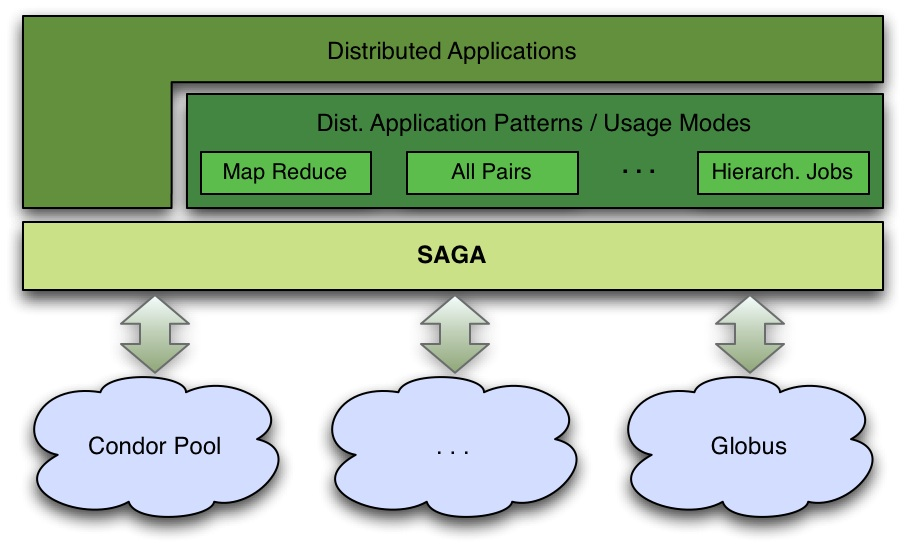
\includegraphics[width=8cm]{sagadistributedappslarge}
\caption{A distributed application running with SAGA, showing how SAGA insulates the application from the heterogeneous nature of multiple distributed resources (from SAGA web-site).}
\end{figure}

\begin{figure}
\centering	
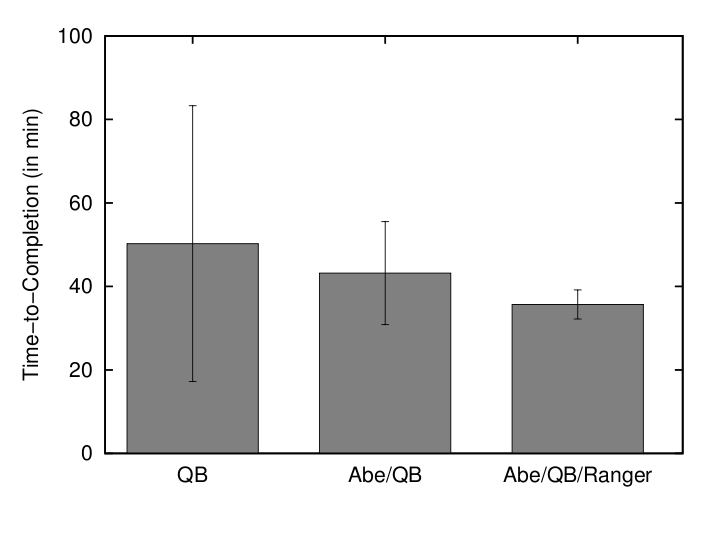
\includegraphics[width=6cm]{namd-rep-size-adaptive}
\caption{A comparison of average time to completion for SAGA/REMD NAMD on three sets of resources (Queen Bee, Abe + Queen Bee, Ranger + Abe + Queen Bee) when the number of processors is adjusted to fit the available resource at run-time.  Reproduced from \cite{ref:saganamd}.}
\end{figure}

\begin{figure}
\centering	
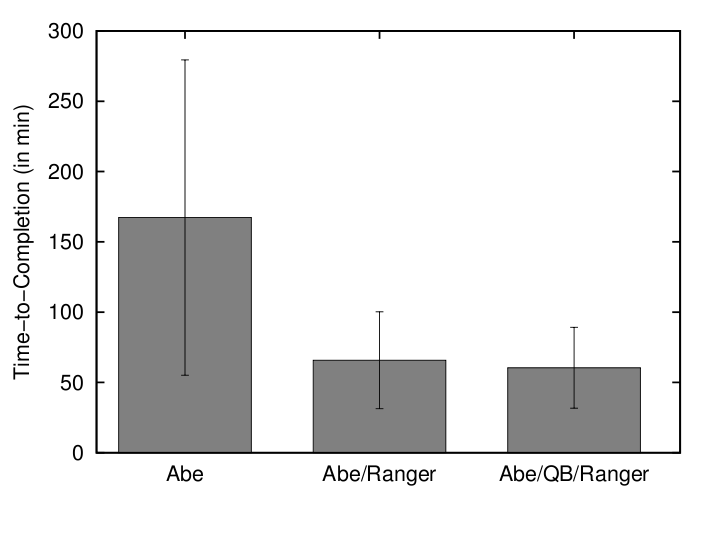
\includegraphics[width=6cm]{namd-rep-num-adaptive}
\caption{A comparison of average time to completion for SAGA/REMD NAMD on three sets of resources (Abe, Abe + Ranger, Ranger + Abe + Queen Bee) when the number of replicas is adjusted to fit the available resource at run-time.  Reproduced from \cite{ref:saganamd}.}
\end{figure}

\thispagestyle{plain}
\begin{thebibliography}{100}
\footnotesize


\bibitem{ref:hpdc} S. Manos, M. Mazzeo, O. Kenway, N. T. Karonis, B. Toonen and P. V. Coveney, Proceedings of High Performance Distributed Computing Boston, Massachusetts, USA, June 23-27 2008

\bibitem{ref:BAC} I. Stoica, S. K. Sadiq, and P. V. Coveney, Journal of the American Chemical Society, 130, (8), 2639-2648, 2008

\bibitem{ref:BAC2} S. K. Sadiq, D. Wright, S. J. Watson, S. J. Zasada, I. Stoica, Ileana, and P. V. Coveney, Journal of Chemical Information and Modeling, 48, (9), 1909-1919, 2008

\bibitem{ref:lammps} S. J. Plimpton, J Comp Phys, 117, 1-19 (1995)

\bibitem{ref:lammps2} S. J. Plimpton, R. Pollock and Mark Stevens, Proc of the Eighth SIAM Conference on Parallel Processing for Scientific Computing, Minneapolis (March 1997).

\bibitem{ref:saganamd} A. Luckow, S. Jha, J. Kim, A. Merzky, B. Schnor,  Phil. Trans. R. Soc. A 28 June 2009 vol. 367 no. 1897 2595-2606

\bibitem{ref:saganamd2} A. Luckow, S. Jha, J. Kim, A. Merzky, B. Schnor,  escience, pp.253-260, 2008 Fourth IEEE International Conference on eScience, 2008

\bibitem{ref:namd} J. C. Phillips, R. Braun, Wei Wang, J. Gumbart, E. Tajkhorshid, E. Villa, C. Chipot, R. D. Skeel, L. Kale, and K. Schulten, Journal of Computational Chemistry, 26:1781-1802, 2005.

\end{thebibliography}

\thispagestyle{plain}
\end{document} 
The volume and complexity of data that must be analyzed in scientific applications is increasing exponentially. Often, this data is distributed; thus, the ability to analyze data by localizing it will yield limited returns. Therefore, an efficient processing of large distributed datasets is required, whilst ideally not introducing fundamentally new programming models or methods. For example, extending MapReduce - a proven effective programming model for processing large datasets, to work more effectively on distributed data and on different infrastructure (such as non-Hadoop, general-purpose clusters) is desirable. We posit that this can be achieved with an effective and efficient runtime environment and without refactoring MapReduce itself. MapReduce on distributed data requires effective distributed coordination of computation (map and reduce) and data, as well as distributed data management (in particular the transfer of intermediate data units). To address these requirements, we design and implement Pilot-MapReduce (PMR) - a flexible, infrastructure-independent runtime environment for MapReduce. PMR is based on Pilot abstractions for both compute (Pilot-Jobs) and data (Pilot-Data): it utilizes Pilot-Jobs to couple the map phase computation to the nearby source data, and Pilot-Data to move intermediate data using parallel data transfers to the reduce computation phase. We analyze the effectiveness of PMR over applications with different characteristics (e. g. different volumes of intermediate and output data). Our experimental evaluations show that the Pilot abstraction for data movement across multiple clusters is promising, and can lower the execution time span of the entire MapReduce execution. We also investigate the performance of PMR with distributed data using a Word Count and a genome sequencing application over different MapReduce configurations.  We find that PMR is a viable tool to support distributed NGS analytics by comparing and contrasting the PMR approach to similar capabilities of Seqal and Crossbow, two Next Generation Sequencing(NGS) Hadoop MapReduce based applications. Our experiments show that PMR provides the desired flexibility in the deployment and configuration of MapReduce runs to address specific application characteristics and achieve an optimal performance, both locally and over wide-area multiple clusters.
\newpage

\pagenumbering{arabic}

%%%%%%%%%%%%%%%%%%%%%%%%%%%%%%%%%%%%%%%%
%New Chapter
%%%%%%%%%%%%%%%%%%%%%%%%%%%%%%%%%%%%%%%%
\chapter{Introduction} 

There are various challenges associated with processing of data at extreme scales: which has become a critical factor in many science
disciplines, e.\,g.\ in the areas of fusion energy (ITER), bioinformatics (metagenomics), climate (Earth System Grid), and astronomy
(LSST)~\cite{Berriman:2011:AAS:2039359.2047483,Jha:2011fk}. The volumes of data produced by these scientific applications is
increasing rapidly, driven by advanced technologies (e.\,g.\ increasing compute capacity and higher resolution sensors) and
decreasing costs for computation, data acquisition and storage~\cite{hey2009}. The number of scientific applications that
either currently utilize, or need to utilize large volumes of potentially distributed data is immense. Recent advances in high-throughput 
DNA sequencing technologies such as  Next-Generation Sequencing (NGS) platforms have resulted in unprecedented challenges 
in the areas of bioinformatics and computational biology~\cite{metzker2010,1000genome,wang2009-natrevgen,alex2009,mcpherson2009}. 
These challenges are to some extent novel because of the need of the cross-cutting and integrated solutions leveraging algorithmic
advances, tools and services, and scalable cyberinfrastructure and middleware.The challenges faced by these
applications are interoperability, efficiently managing compute tasks, and moving data to the scheduled compute location.

%Intro to MapReduce

Processing large volumes of data is a challenging task. MapReduce is an effective programming model for addressing this challenge. MapReduce involves two 
major computation phases called map and reduce, separated by a shuffle phase, which involves movement of intermediate data. 
MapReduce starts with chunking of the input data with user configured chunk size and assign each chunk to a single user defined mapper function in map phase. Once the map phase is completed i.e., when all the mapper functions completed, the output of map phase is scattered equally to the reduce phase based on a partitioning function. The reduce phase involves gathering of input data relavent to a reduce and execute the user defined reducer function on the data. MapReduce~\cite{Dean:2004:MSD:1251254.1251264} as originally developed by Google aims to address the big data problem by providing an
easy-to-use abstraction for parallel data processing. The most prominent framework for doing MapReduce computations is Apache
Hadoop~\cite{hadoop}. However, there are limitations to the current MR implementations: (i) They lack a modular architecture, (ii) are
tied to specific infrastructure, e.\,g.\ Hadoop relies on the Hadoop File System (HDFS), and (iii) do not provide efficient support for
dynamic and processing distributed data, e.\,g.\ Hadoop is designed for cluster/local environment, but not for a high degree of
distribution.

Pilot abstractions enable the clean separation of resource management concerns and application/frameworks. In particular, \pilotjobs 
have been notable in their ability to manage large numbers of compute units across multiple high performance clusters, providing decoupling
application-level scheduling and system-level resource management. But, there is also a need of an abstraction to liberate
applications from the challenging task of compute-data placement and scheduling. The Pilot-API~\cite{pstar-2012} aims to address this issue
by providing a unified API for managing both compute and data pilots. \emph{BigData (BD)} is an extension of
the BigJob framework (BJ)~\cite{bigjob_web} to data. Both BigJob and BigData provide a full implementation of the Pilot-API and enable the
management of resources, compute \& data units as well as the relationships between them. Specifically, the Pilot-API promotes
affinities as a first class characteristic for describing such relationships between compute and data elements and to support dynamic
decision making. 

A critical aspect of MapReduce, is the management of data and compute localities as well as the management of data movements, e.\,g.\
between the map and the reduce phase.  In this thesis, we demonstrate the efficient support of these capabilities via the Pilot
abstractions. We design and implement \pilotmapreduce \ -- a novel \pilot-based MapReduce implementation which enables clean separation
of resource management and MapReduce application. Our \pilotmapreduce framework demonstrates how \pilot abstractions are used for managing the map and reduce tasks and
intermediate shuffle data between them and the advantages of the \pilot-based architecture in terms of flexibility,
extensibility, scalability and performance; for example, we discuss the usability of \pilot-abstractions in designing dynamic execution
workflows which involves multiple MapReduce computations.

Before we proceed further, it is critical to emphasize that it is not the aim of this thesis to suggest PMR as a replacement to Hadoop.
However, we posit that where MR-based applications need to be employed over distributed data, including but not limited to clusters connected
over WAN, or production distributed cyberinfrastructure such as XSEDE, EGI, PMR provides a flexible, extensible implementation of MR that is
also efficient.

At this point, I would like to clarify my contribution to this work. The Pilot-API was developed in ~\cite{pstar-2012}. 
I used this Pilot-API to develop the MapReduce framework. I evaluated the performance and scalability of the different  
MapReduce configurations using the Word Count application on natural language and on random data as well as the 
genome sequencing application. We have submitted this work for two publications and the drafts can be accessed here ~\cite{ecmls-2012, mrworkshop-2012}.
 
This thesis is organized as follows: Chapter ~\ref{chap:pilot-bg} gives an overview of \pilot
abstractions. In Chapter~\ref{chap:pilot-mr} we discuss the design and implementation of the \pilotmapreduce framework.
In Chapter~\ref{chap:pilot-app} we evaluate the performance and scalability  of  \pilotmapreduce.
Chapter ~\ref{chap:pilot-lasigma} gives performance evaluation of BigJob on XSEDE and LONI. The conclusion and future work are given in Chapter ~\ref{pilot-conclusion}.

\chapter{Pilot Abstractions} \label{chap:bg}

In this section we describe some of the different components of Pilot Abstractions that are important for understanding this work, and their application and 
importance on distributed cyber infrastructure. 

First, in Section~\ref{sec:ci} we will describe the distributed cyber-infrastructure,  In Section~\ref{sec:trad-cd-mgmt} we focus on the traditional job submission methodologies and their problems. 
 In Section~\ref{sec:pa} we describe the Pilot Abstractions and their implementation for both compute and data . In Section~\ref{sec:pilot-sol-ci} we describe how Pilot-Jobs and Pilot-Data provide
effective management of distributed cyber-infrastructure.

\section{Distributed Cyber-Infrastructure} \label{sec:ci}

Distributed cyber-infrastructure(DCI), in contrast to a static resource utilization model utilizes computing resources, which varies in load and capability.
Domain Scientists understand scientific applications related to their field by experimenting on DCI. Some of the requirements and characteristics of these 
applications require broad usage of DCI which are significant different from regular HPC aplications in sevaral fundamental ways. Often, distributed applications 
are designed to support peak utilization of resources by a number of tasks. On distributed dynamic resource pool, it is an important attribute of any application to
utilize the infrastructure efficiently. Production Grid Infrastructures (PGIs) as well as the Programming Systems and Tools (PS\&T) used to develop distributed 
applications need to address these and other fundamental distributed application characteristics ~\cite{bigjob-1}.

\section{Traditional compute and data management} \label{sec:trad-cd-mgmt}

Existing PS\&T support number of applications to utilize DCI. Even though several distributed applications use distributed infrastructures sucessfully, either those applications failed to use distributed infrastructures effectively or have had to implement new capabilities at one or more levels, which includes application, programming system, middleware and/or infrastructure level.  The urge to utilize distributed infrastructures effectively made the design and development of distributed applications more complex task~\cite{bigjob-2}. For example, many programming systems and tools for distributed applications are either incomplete and/or often out-of-phase with requirements or inflexible with respect to application needs, e.g. tools that support the master-worker paradigm often only address failures of workers and not of the master. Additionally, tools and development systems often don't support the specific usage modes that maybe required for a certain application scenario, with the level of robustness and scalability required, i.e., solutions work well in small or controlled environments, but not at-scale.  These and other concerns have motivated developers to "roll out their own" capabilities, in turn further adding to an existing large range of tools, programming systems and environments and adding to challenges of providing interoperability. Thus to the extent possible, extensibility and interoperability must be built as fundamental design objective of PS\&T for distributed applications and infrastructure.  Although it will not be possible to support all of the following properties, PS\&T should address some of these aspects: (i) new application domains and usage-modes, (ii) extending the functionality supported, (iii) extension to new infrastructures, (iv) extend across scales of opera- tion, (v) uptake by communities other than the developer (community usage) and, (vi) reuse and support patterns and abstractions for distributed computing.  The extend to which the above design objectives will succeed depends not only on the resulting programming system, but also on the availability of usable and extendable abstractions and their suitability for given production infrastructures. Interestingly, the Pilot-Job abstraction has been widely used across several different PGIs. However, the existing Pilot-Job frameworks are all heavily customized and often tightly coupled to a specific infrastructure, and not extensible or usable across different systems, e.g. there is no such "unifying" and "extensible" Pilot-Jobs that supports a range of application types and characteristics. ~\cite{bigjob-1,bigjob-2}

Many scientific applications have immense data requirements, which are projected to increase dramatically in the near future ~\cite{pstar-32}.  The management of data in distributed systems remains a challenge due to various reasons: (i) the placement of data is often decoupled from the placement of Compute Units i. e. the application must often manually stage in and out its data using simple scripts; (ii) heterogeneity, e. g. with respect to storage, filesystem types and paths, often prohibits or at least complicates late bind- ing decisions; (iii) higher-level abstraction that allow applications to specify their data dependencies on an abstract, logical level (rather than on file basis) are not available; (iv) due to lack of a common treatment for compute and data, optimizations of data/compute placements are often not possible. In addition, applications must cope with various other challenging, data-related issues, e.g. varying data sources (such as sensors and/or other application components), fluctuating data rates, transfer failures, optimizations for differ- ent queries, data-compute co-location etc. While these issues can be in principal handled in an application-specific way, the usage of higher-level abstractions, such as a common Pilot-based abstraction for compute and data is preferable.


\section{Pilot abstractions for compute and data} \label{sec:pa}
Pilot-abstractions provide effective management of compute and data units and the relationships between them(affinities). They liberate the applications from the challenging require- ment of assigning/scheduling the compute or data unit onto a particular resource.

\subsection{BigJob - SAGA Pilot Job} \label{sec:pj}
The abstraction of a Pilot-Job (PJ) generalizes the reoc- curring concept of utilizing a placeholder job as a container for a set of compute tasks; instances of that placeholder job are commonly referred to as Pilot-Jobs or pilots. The PJ provides applications (user) level control and management of the set of allocated resources.
BigJob (BJ) is a SAGA-based PJ framework. BJ has been designed to be general-purpose and extensible. While BJ has been originally built for HPC infrastructures, such as XSEDE and FutureGrid, it is generally also usable in other environments. This extensibility mainly arises from the usage of SAGA as a common API for accessing distributed resources. SAGA provides a simple, POSIX-style API to the most common grid functions at a sufficiently high-level of abstraction so as to be independent of the diverse and dynamic grid environments. ~\cite{bigjob-15}

\subsection{BigData - SAGA Pilot Data} \label{sec:pd}
Analogous to Pilot-Jobs, Pilot-Data(PD) provides late-binding capabilities for data by separating the allocation of physical storage and application-level data units [15].
BigData (BD) is an implementation of the Pilot-Data ab- straction. BigData is designed to work together with BigJob (BJ) [18] - a SAGA-based Pilot-Job implementation. Fig- ure 1 gives an overview of the architecture. The system consists similarly to BigJob of two components: the BD- Manager and the BD-Agents deployed on the physical re- sources. The coordination scheme used is again M/W with some intelligence that is located de-centrally at the BD- Agent. As communication mechanism the SAGA Advert Service is used, in a similar push/pull mode as for BJ. The BD-Manager is responsible for (i) meta-data manage- ment, i. e. it keeps track of the pilot stores that a pilot data object is associated with, (ii) for scheduling data movements and data replications (taking into account the application requirements defined via affinities), and (iii) for managing data movements activities. For this purpose, it can rely on external service, e. g. Globus Online for data transfer man- agement. Similar to BigJob, an agent on each resource is used to manage the physical storage on a resource. A particular critical requirement for data-intensive application, is the management of affinity between CUs and also between DUs and DUs. The BD scheduler supports preliminary affinity-aware scheduling: both BigJob and BigData are tightly integrated to efficiently support compute- and data-related aspects of dynamic execution.

\subsection{Pilot API and Affinities} \label{sec:pilot-api}
The Pilot-API is an interoperable and extensible API which exposes the core functionalities of a Pilot framework via a unified interface providing a common API that can be used across multiple distinct production cyber infrastructures. The API provides three core classes: the PilotCompute- Service for the management of Pilot-Jobs, PilotDataService for the management of Pilot-Data and the Compute- DataService for the management of ComputeUnits (CUs) and DataUnits (DUs). A CU represents a primary self- containing piece of work, while a DU represents a logical set for data [15].

The Pilot-API promotes affinities as a first class character- istic for describing relationships between data and/or com- pute supporting dynamic decision making. Unfortunately, most production infrastructure lack system-level support for affinities, e. g. resource localities cannot be introspected. Data storage in particular in distributed settings, such as in the XSEDE or the EGI environment, is often a black box for the application with unknown quality of services, i. e. the application usually does not know what bandwidths and la- tencies it can expect. To address these deficiency the Pilot- API introduces affinities on application-level: applications can associate compute and data units as well as resources (the Pilots) with affinity labels. The BigJob and BigData runtime will then ensure that CUs and DUs are placed with respect to the affinity requirements of the application.

\section{Scalability and Usability of Pilot Abstractions} \label{sec:pilot-sol-ci}
Pilot abstractions have been proved to provide effective scaling at various levels ~\cite{repex,pstar, bigjob} and they can be defined as
\begin{itemize}
\item{scale-up: Refers to the ability (performance) of using many cores efficiently}
\item{scale-out: Measures the number of tasks that can be concurrently executed \& managed}
\item{scale-across: Measures the number of distinct compute homogenous or heterogenous resources  that an application can utilize.}
\end{itemize}

We demonstrate the usability of Pilot-abstractions to design a flexible, infrastructure-independent runtime environment for MapReduce application. Pilot-MapReduce heavily relies on Pilot abstractions for de-coupling the MapReduce runtime, application-level scheduling and resource management providing a high degree of flexibility and extensibility.

\section{Architecture of \pilotmapreduce} \label{sec:pilot-mr}
\pilotmapreduce introduces a clean separation of concerns between
compute and data management on the one hand, with their scheduling in
a distributed context. The pilot abstraction enable the easy
acquisition of both compute and storage resources. The \mrmg can
focus on orchestrating this resource pool. This architecture can also
efficiently support workloads that currently not supported well
enough by Hadoop, e.\,g.\ iterative
applications. Figure~\ref{fig:figures_mapreduce-pilotdata} shows the
architecture of the \pilotmapreduce framework.

\begin{figure}[t]
	\centering
	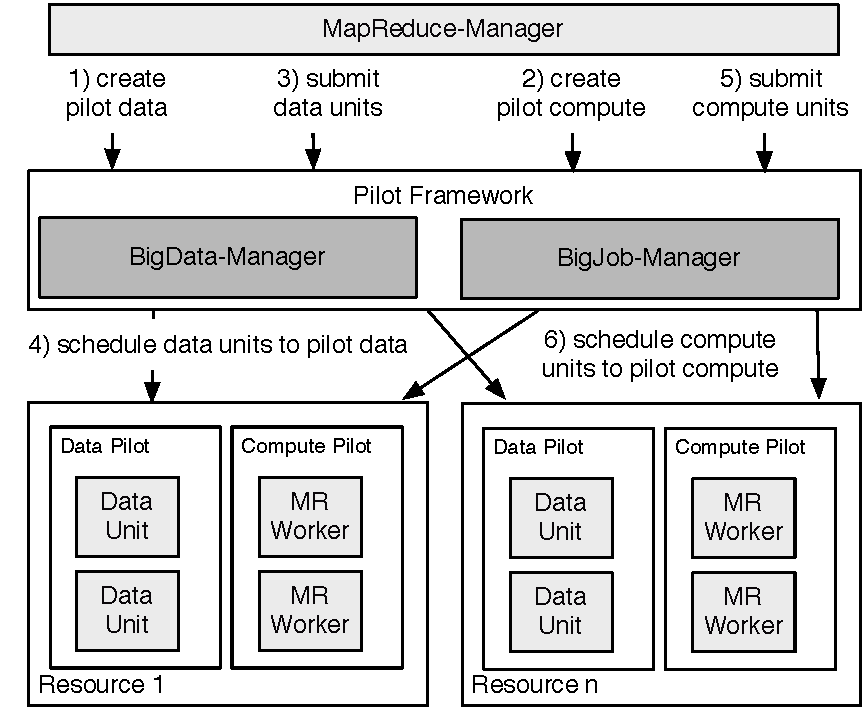
\includegraphics[width=0.38\textwidth]{figures/mapreduce-pilotdata.pdf}
	\caption{\textbf{Pilot-based MapReduce:} Each pilot (both compute and data 
	pilot) can be associated with an affinity label. The BigData and BigJob 
	Manager will ensure that CUs and DUs are placed with respect to these 
	requirements.\upp}
	\label{fig:figures_mapreduce-pilotdata}
\end{figure}

The flow of a typical MapReduce application involves the chunking of
the data, the execution of the map compute tasks, shuffling and moving
the intermediate data to the reduce task and finally the execution of
the reduce tasks.  \pilotmapreduce utilizes a set of compute and data
pilots for this application workflow: 
\upp
\begin{compactenum}[A.]
\item Initially, the \mrmg allocates a set of compute and data
  resources by starting one (or most often a set of) compute and data
  pilots on different resources.  In general, on each resource one
  compute and one data pilot is co-located. The data pilot is either
  created with reference to local input data or the input data is
  moved to the data pilot after its creation.


\item \textbf{Chunking:} % \pnote{commented - The input data on each resource is
% {\it chunked}.}
The \mrmg executes a \cu on each resource, which splits the
input data on the respective resource with respect to the defined chunk
size.\label{stp:chunking} 
Each chunk is stored in a new DU. BigJob and BigData -- in particular
the \texttt{ComputeDataService} -- are used as the common abstraction
for managing the \computeunits and \dataunits. 
  

\item \textbf{Mapping:} The \mrmg assigns a {\it map} CU to each
  chunk created in step~\ref{stp:chunking}. Again, BJ is used for
  managing the CUs. BJ and BD ensures that each CUs is co-located with
  an appropriate DU taking into account data localities and minimizing
  the amount of data movements.

\item \textbf{Shuffling:} 
  After the map phase is completed the output data is sorted and
  partitioned. For each partition a \du is created. Each partition is
  then processed by a reduce task. For this purpose, the \mrmg assigns
  each reduce CU to a DU. Each DU comprises of a group of sorted,
  partitioned map output files. \cus and \dus are then submitted
  through the \texttt{ComputeDataService} of BJ and BD. The
  affinity-aware scheduler ensure that \cus are assigned to local \dus
  minimizing the amount of data transfers. 	For each reduce task a 
  Data Unit containing the necessary input files is created and submitted. % (step 3/4 in
  %figure~\ref{fig:figures_mapreduce-pilotdata})



	
\item \textbf{Reducing:} The {\it reduce} tasks are prepared and
  executed on the DUs representing the intermediate data.
  % (step  5/6 in figure~\ref{fig:figures_mapreduce-pilotdata}).  
  The management of the data transfers is done by BJ/BD taking into account the 
  specified affinities.
	
\item The \pilots are terminated.

\end{compactenum}
\upp


The Pilot-API provides a well-defined abstraction for supporting the
late-binding of compute and data units decoupling resource assignment
from resource usage. Using BJ and BD, PMR can allocate both storage
and compute resources, which can then be flexibly utilized for
executing map and reduce tasks as well as for storing both
intermediate and output data.

The API also allows the expression and management of relationships
between data units and/or compute units. BigJob and BigData provide an
implementation of the Pilot-API. These frameworks ensure that the data
and compute affinity requirements of the MapReduce applications are
met for each step of the MapReduce workflow. For example, in the
shuffle phase for each reduce task a DU and CU is generated. These are
then submitted to BigJob and BigData framework, which handles the
scheduling, transfer of the DU and execution of the CU. PMR assigns a
resource affinity to each DU and CU. BJ and BD then ensure that each
CU is co-located to the right DU.

\upp
\subsection{Compute and Data Management}
The PMR relies on the master/worker coordination model, i.\,e.\ a
central MapReduce-Manager is responsible for coordinating the
MapReduce workers, which in turn are responsible for executing map and
reduce tasks. The MapReduce-Manager utilizes BigJob and BigData for executing
mapper and reduce tasks (Listing~\ref{lst:pcs_creation}).


\lstset{
language=Python,
frame=single,
captionpos=b,
stringstyle=\ttfamily,
basicstyle=\scriptsize\ttfamily
}
\noindent\begin{minipage}{1 \textwidth}
\begin{lstlisting}[caption={\textbf{Pilot Compute Creation:} Instantiation of a Pilot Job using Pilot Compute Description}, label={lst:pcs_creation}]
pcs = PilotComputeService()
cds = ComputeDataService()
pjd ={"service_url":"pbs-ssh://sierra.futuregrid.org", 
"number_of_processes": '8',
"walltime":10, 
"processes_per_node:'8',
"affinity_datacenter_label":'sierra',
"affinity_machine_label":'sierra'}
pj=pcs.create_pilot(pilot_compute_description=pjd)
cds.add_pilot_compute_service(pcs)
\end{lstlisting}
\end{minipage}

Similarly, Hadoop also utilizes a job and task tracker: the job
tracker is the central manager that dispatches map and reduce tasks to
the nodes of the Hadoop cluster. On each node the task tracker is
responsible for executing the respective tasks. The main limitation of
this architecture is the fact that it intermixes both cluster resource
management and application-level task managements. Thus, it is not
easily possible to integrate Hadoop with another resource management
tool, e.\,g.\ PBS or Torque. Also, the job tracker represents a single
point of failure and scalability bottleneck.

% \subsection{Data Management in \pilotmapreduce}

The efficiency of PMR in particular on multiple resources depends on
the management of the the intermediate data. BigData not only
provides flexibility to manage the relationship between data and
compute units, but also allows {\it parallel} data transfers between
machines and between data units.  BigData is used for moving the
intermediate output files of the mapper tasks to the resource where
the reduce compute units are executed.  Listing~\ref{lst:pds_creation}
illustrates the creation of a new Pilot-Data at the location of the
reduce task.

\lstset{
language=Python,
frame=single,
captionpos=b,
stringstyle=\ttfamily,
basicstyle=\scriptsize\ttfamily
}
\noindent\begin{minipage}{1 \textwidth}
\begin{lstlisting}[caption={\textbf{Pilot Data Creation:} Instantiation of a Pilot Data using Pilot Data Description}, label={lst:pds_creation}]
pds = PilotDataService()
pd_desc=
{"service_url":"ssh://india.futuregrid.org/pilotdata",
"size":100,
"affinity_datacenter_label":'india',
"affinity_machine_label":'india'}
pd=pds.create_pilot( pilot_data_description=pd_desc)
cds.add_pilot_data_service(pds)
\end{lstlisting}
\end{minipage}

\upp
\subsection{Distributed MapReduce}
\label{sec:pmr-distributed}
An increasing amount of data that scientific applications need to
operate on is distributed. Often data generation
and processing are far apart: For example, the Earth Science Grid
federates data of various climate simulations~\cite{ESG}. Meta-genomic
workflows need to process and analyze data generated by various
sequencing machines~\cite{Jha:2011fk}; the localization onto a single
resource is often not a possibility.

Several options for running Hadoop on distributed data have been
proposed~\cite{weissman-mr-11}: (i) in a global MapReduce setup one
central JobTracker and HDFS NameNode is used for managing a
distributed set of resources; (ii) in a hierarchical MapReduce setup
multiple MapReduce clusters are used: a MapReduce cluster close to the
data source for pre-processing data and a central cluster for
aggregating the different de-central data sources. The volume of the
pre-processed data is generally lower and thus, can be easily moved to
another processing resource. 

Ref.~\cite{weissman-mr-11} shows that a hierarchical Hadoop
configuration leads to a better performance than a naive global Hadoop
cluster for some application. A main drawback of this approach is the
increased complexity: Hadoop is not designed with respect to a
federation of multiple MapReduce clusters. Thus, setting up such a
system requires a lot of manual effort.  \pilotmapreduce in contrast
utilizes the Pilot-API as a unified abstraction for compute and data
resources; thus MapReduce framework can be used to reason about data
and compute localities and is able to operate on a dynamic and
distributed pool of storage and compute resources.


\begin{figure}
	\centering
	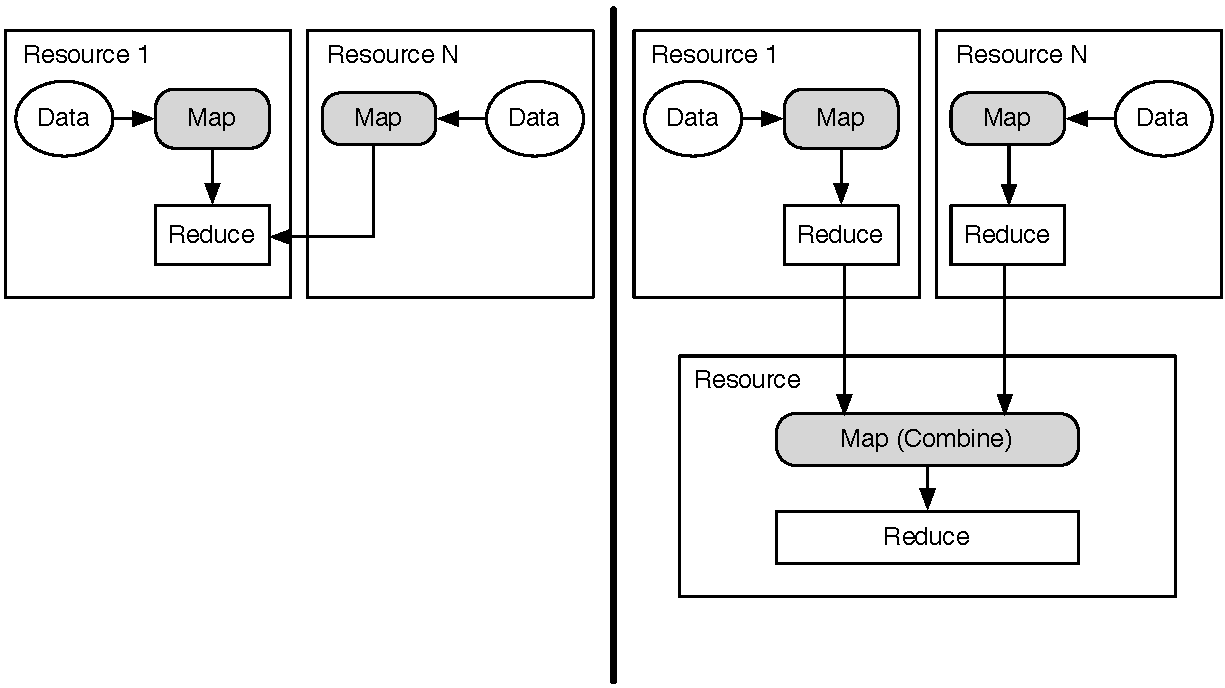
\includegraphics[width=0.48\textwidth]{figures/distributed_hierachical.pdf}
	\caption{\pilotmapreduce Deployment Scenarios: In the
          distributed scenario (left), the mapping tasks are run close
          to the data, the reduced tasks are then run on a single
          resource. In the hierarchical scenario (right) two complete
          MapReduce runs are
          conducted. \label{fid:distributed-mapreduce-overview}}
\end{figure}


\pilotmapreduce supports different distributed MapReduce topologies:
(i) \emph{local}, (ii) \emph{distributed} and (iii)
\emph{hierarchical}. A local PMR performs all map and reduce
computations on a single resource.
Figure~\ref{fid:distributed-mapreduce-overview} shows options (ii) and
(iii): A distributed PMR utilizes multiple resources often to run map
tasks close to the data to avoid costly data transfers; the
intermediate data is then moved to another resource for running the
reduce tasks. BigJob and BigData are used for managing CUs and DUs and
the necessary data movements. In contrast, in a hierarchical PMR the
outputs of the first complete MapReduce run are moved to a central
aggregation resource. A complete MapReduce run is then executed on
this resource to combine the results.

The Pilot-API provides a consistent API for managing both compute units (i.\,e.\ 
map and reduce tasks) and data units. Using descriptive affinities label the  
data flow between CUs, i.\,e.\ the transfer of the intermediate data, can be 
efficiently managed. Using this capability PMR can be easily scaled out to 
multiple resources to support scenarios (ii) and (iii). 

%%%%%%%%%%%%%%%%%%%%%%%%%%%%%%%%%%%%%%%%
%New Chapter
%%%%%%%%%%%%%%%%%%%%%%%%%%%%%%%%%%%%%%%%
\chapter{Evaluation of \pilotmapreduce} \label{chap:pilot-app}

In this section we analyze the performance and scalability of
\pilotmapreduce and compare it to Hadoop MapReduce using different
applications. For this purpose we run several experiments on
FutureGrid~\cite{fg}. We run the experiment on the following
FutureGrid resources: India, Sierra and Hotel. Each experiment is
repeated at least three times. For our Hadoop experiments, we use
Hadoop 0.20.2. At the begin of each run a Hadoop cluster is started
via the Torque resource management system on a specified number of
nodes. The first assigned node is used as master node running the
Hadoop JobTracker and the NameNode. The HDFS replication factor is set
to 2 and number of reduces to 8.
\upp
\subsection{MapReduce-Based Applications}

MapReduce has been utilized in various science applications. A key performance 
factor is the amount of data that must be moved through the MapReduce system. 
The degree of data aggregation of the map tasks is thus, an important 
characteristic of a MapReduce application~\cite{weissman-mr-11}.

MapReduce application can be classified with respect to different
criteria: (i) the volume of the intermediate data (i.\,e.\ the size of
the output of the map tasks), and (ii) the volume of the output data,
(i.\,e.\ the size of reduce phase output), and the relative proportion
of these data volume. In the following we investigate two application
scenarios: Word Count and a Genome Sequencing application.

\upp
\subsubsection*{Word Count}

The Word Count application is the basis for many machine learning use cases, 
used e.\,g.\ for the classification of documents or clustering. Word Count 
generates a large volume of intermediate data ($\sim$200$\%$). The volume of the 
output data depends on the type of input data, e.\,g.\ the size of the output data is 
larger for a random input than for an input in a natural language. 

\upp
\subsubsection*{Genome Sequencing (GS)}

High-throughput genome sequencing techniques provided by Next Generation
Sequencing (NGS) platforms are changing biological sciences and biomedical
research. The data volumes generated by sequencing machines is increasing
rapidly. The distributed processing of this data requires a sophisticated
infrastructure. For this purpose, we utilize MapReduce to model an important
part of the sequencing workflow i.e, the read alignment and the duplicate
removal. 

\subsubsection*{Short Read Alignment}

Short reads alignment and the de-novo assembly are the required first
steps in every pipeline software tool that aims to analyze sequencing
data from NGS platforms.  De-novo assembly still remains a challenge,
because of complications arising from the short length of sequencing
reads from NGS machines. In most of situations, read alignment (or mapping process)
is the first task of NGS workflows, and two Hadoop-based tools, Seqal and Crossbow provided two mapping tools, BWA and Bowtie, respectively. 

In general, for RNA-Seq data analysis, in particular with eukaryote
genomes, the spliced aligner such as TopHat~\cite{pepke2009} is
used. In our work, we consider an alternative strategy, to use a
non-spliced aligner and later splicing events are detected separately,
justifying the use of non-spliced aligners such as BWA and Bowtie for
the RNA-Seq data.  These non-spliced aligner tools mapped reads onto human reference genome hg19.

\subsubsection*{Post-Alignment}
Duplicate read removal step might be required after short read
alignment, because sample preparation processes before sequencing
might contain artifacts stemming from high-throughput read
amplification; many duplicates introduced are not relevant to true
biological conditions. 

Seqal is a Hadoop MapReduce application which implements the alignment
in map phase using BWA aligner and a duplicate removal step using the same criteria as the Picard
MarkDuplicates~\cite{seal2011,seal_2011_mapred} in reduce phase. 
We use two implementations of the workflow: the Hadoop-based 
Seqal~\cite{seal-2011} application and a custom implementation of this workflow 
GS/PMR. Both application implement the read alignment in the mapping phase of 
the application using BWA aligner~\cite{Li:2010:FAL:1741823.1741825}. In the 
Seqal case the duplicate removal in the reduce phase is implemented using  
Picard's rmdup~\cite{picard}. The GS/PMR reduce phase is not an exact implementation of
Seqal's Picard rmdup implementation.We developed a custom script in python
which is based on duplicate removal description provided in ~\cite{seal-2011}. 
The GS/PMR reducer removes duplicate reads based on the key fields-chromosome,
position, strand of GS/PMR mapper output.

Crossbow ~\cite{langmead2009} is a scalable software automatic pipeline, combines Alignment and SNP finding tools for DNA sequencing analysis.
Crossbow contains 4 steps - preprocessing, Alignment, SNP finding and postprocessing.  Each step is a Hadoop streaming-based MapReduce application and the output of each step is stored in HDFS and read from HDFS by the next step.  In our experiments we focused on Crossbow alignment which uses Bowtie aligner in map phase and has a dummy reducer.  


%%%%%%%%%%%%%%%%%%%%%%%%%%%%%%%%%%%%%%%%%%%%%%%%%%%%%%%%%%%%%%%%%%%%%%%%%%%%
\upp
\subsection{Characterizing Word Count}


In the first experiment, we benchmark the performance of
\pilotmapreduce and Hadoop using a simple Word Count application on a
single resource. For both frameworks, 8 nodes on India machine are
used. In all scenarios the input data is pre-staged on the respective
resources, i.\,e.\ for Hadoop the data is located in HDFS, for PMR the
data is stored on a shared file system. We set the total number of
reduces to 8 for both Hadoop and \pilotmapreduce; further, the default
chunk size of 128\,MB is used. A HDFS replication factor of 2 is used.

The runtime of PMR includes the time to chunk input data, running the
mapping CUs, shuffling (which again comprises of sorting and the
intermediate data transfer, and finally running the reduce CUs.
Figure~\ref{fig:figures_wc_pmr_hmr} shows the results. The runtime of
Hadoop MapReduce includes the time to load input source data into HDFS and
MapReduce runtime.

\begin{figure}[ht]
	\centering
		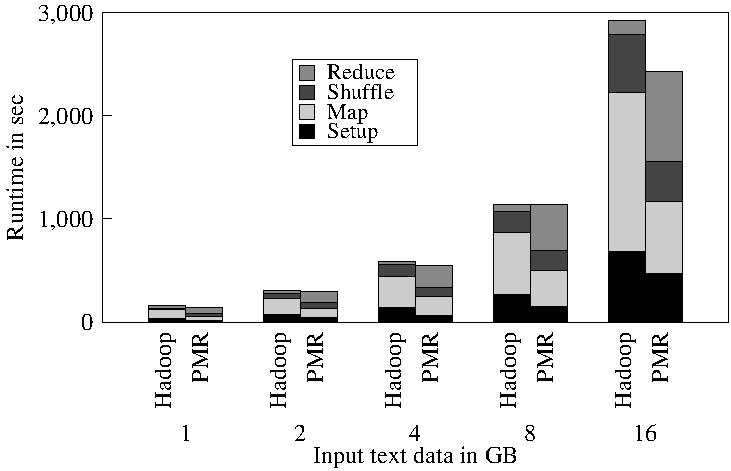
\includegraphics[width=0.47\textwidth]{figures/wc_pmr_hmr.pdf}
                \caption{Word Count PMR vs. Hadoop: The performance of
                  Hadoop and PMR is comparable. The runtime increase
                  with the input data size. Hadoop tasks have a
                  notable higher startup time.\upp}
\label{fig:figures_wc_pmr_hmr}
\end{figure}		
	
The time to solution increased linearly as data size increased; the
performance of both Hadoop and PMR is comparable up to 8\,GB. However,
for the largest volumes of input data we examined, PMR shows a better
performance than Hadoop. In particular, the setup, map and shuffle phase in the 
Hadoop case are longer. Both the map and shuffle phase are the most  
data-intensive phases -- Word Count needs to read all input files and generates 
intermediate data with the size of about 200\,\% of the input data. The worse 
performance of Hadoop indicates a potential issue with HDFS. PMR relies mostly 
on the shared file system for handling the intermediate data.


\upp\upp
\subsection{Characterizing Genome Sequencing}

In this section, we compare and contrast GS/PMR and Seqal. For both
applications, we utilize the same set of input data comprising of different
sizes of read files and the reference genome. Seqal, however, expects the input
data in a different format (prq instead of fastq); thus, the data was previously
converted to meet the Seqal requirements. For PMR, the fastq files from
sequencing machines are directly used; further, a custom chunk script is used to
chunk the fastq files based on the number of reads. We make sure that the chunk
size for both Seqal and PMR is equal. For both frameworks, a total of 4 nodes on
FutureGrid Sierra machine, 8 reduces, 2 workers/node, default chunk size of
128\,MB is used. For Hadoop based Seqal, the replication factor of two is used.
Since Seqal and GS/PMR utilize different duplicate removal tools in the reduce
phase, we focus our investigation on the map phase.


\begin{figure}[ht]
	\centering
		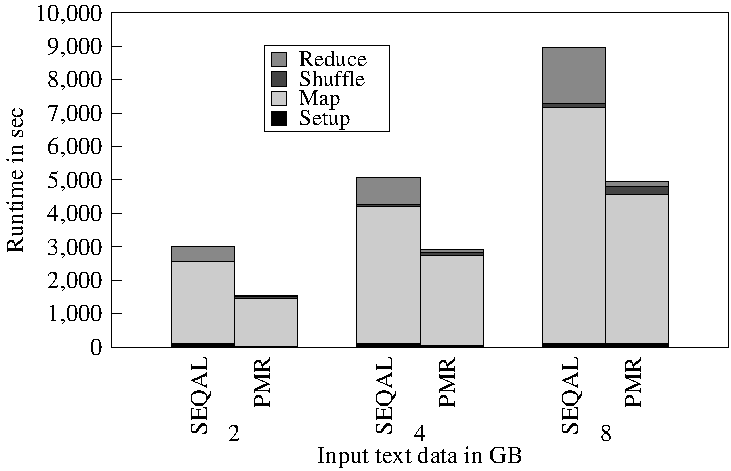
\includegraphics[width=0.47\textwidth]{figures/gs_seq_pmr.pdf}
\caption{Seqal and GS/PMR: GS/PMR provides a marginal better performance that 
Seqal. The overhead of Seqal is mainly attributed to the used HDFS configuration 
using a shared file system.\upp} 	
\label{fig:gs_seq_pmr}
\end{figure}		

Figure~\ref{fig:gs_seq_pmr} shows the results of both applications. In the setup
time of Seqal, Hadoop copies the reference genome archive to all the nodes and
extracts it so it is available locally. In comparison to Word Count both GS
applications are more compute intensive, i.\,e.\ the ratio between computation
in the map phase and the size of the input data is significant larger. Notably,
Seqal requires a longer time-to-completion than GS/PMR. Both the map and reduce
phase of Seqal are longer. While the map phase of Seqal relies on the same BWA
implementation as GS/PMR, the reduce phase uses Picard's rmdump~\cite{picard}
for duplicate removal, which has a significant longer runtime than the duplicate
removal process in the reduce phase of GS/PMR.

This is mainly caused by a non-optimal configuration of Hadoop: The local disks
available on FutureGrid is too small for the used input data; thus, HDFS had
to be configured to utilize a shared, distributed file system, which
leads to a non-optimal performance during the I/O intensive map
phase. The difference in the reduce phase mainly originate from the
different implementations of the duplicate removal process in Seqal
and GS/PMR.

\upp\upp
\subsection{Distributed and Hierarchical MapReduce}

In this section, we evaluate the performance and scalability of the
(i) distributed and (ii) hierarchical PMR configuration (see
section~\ref{sec:pmr-distributed}) using the Word Count application on
natural language and on random data as well as the genome sequencing
application. In the distributed scenario (i) the map CUs are
distributed across two machines, in the hierarchical scenario (ii) two
resources are used each executing an independent MR run. The MapReduce
run for combining and aggregating the output of the first round is
executed on one of these machines. The performance of each application
depends on the amount of generated intermediate and output
data.  Table~\ref{tab:data-volumes} summarizes the characteristics of
the used applications.

\begin{table}[ht]
	\centering
\begin{tabular}{|p{2cm}|c|c|c|}
\hline
\textbf{Application} &\textbf{Input} &\textbf{Intermediate} &\textbf{Output}\\
\hline
GS/PMR 		&80\,GB &71\,GB		 &17\,GB\\
\hline
Word Count\linebreak[4] (English) &16\,GB&26\,GB&20\,MB\\
\hline
Word Count (random) &16\,GB&30\,GB&30\,GB\\
\hline
\end{tabular}
\caption{Data Volumes for different Applications\upp}
\label{tab:data-volumes}
\end{table}

\upp\upp
\subsubsection{Word Count}

For Word Count we compare a distributed and hierarchical PMR
configuration with the performance of two Hadoop configurations: a
single resource Hadoop configuration (half of the data is initially
moved to that cluster) and a hierarchical Hadoop setup with two
resources. We utilize two machines, Sierra and Hotel. The initial
input data of 16\,GB is equally distributed on these two machines. As
mentioned, for the single resource Hadoop configuration half of the
input data needs to be moved from Sierra to Hotel prior to running the
actual MapReduce job. Unfortunately, the FutureGrid firewall rules
prohibited the usage of a distributed Hadoop setup. For all
configurations, we use 8 nodes.

Figure~\ref{fig:allmrs_rands} shows the results. For natural language
input, both Hadoop and PMR show a comparable performance. A major
performance factor for Hadoop in the case of distributed data is the
necessity to move parts of the data (half of the input data) to the
central Hadoop cluster. The performance of PMR is determined by the
runtime of the map and reduce phase, which are slightly longer than
for Hadoop mainly due to the resource heterogeneity and the resulting
scheduling overhead: the slowest node determines the overall runtime
of both the map and reduce phase.

Both the hierarchical Hadoop and PMR perform better than the
distributed PMR and single resource Hadoop configuration. The
performance is mainly influenced by the data that needs to be
moved. In the distributed case half of the intermediate data needs to
be moved to the other resource; in the hierarchical case half of the
output data requires movement. Since the output data in the
hierarchical case is a magnitude smaller than the intermediate data in
the distributed case (cmp. table~\ref{tab:data-volumes}) -- 20\,MB in
comparison to 30\,GB -- the performance in the hierarchical case is
significant better.

For random data, the distributed PMR and single resource Hadoop perform better
than the hierarchical PMR and Hadoop configuration. In this case the output data
is about equal to the intermediate data (30\,GB), i.\,e.\ the advantage of a
reduced transfer volume does not exit. In this case the additional MapReduce run
represents an overhead. In the Hadoop case, the moved data needs to get loaded 
into HDFS, which represents another overhead.


\begin{figure}[ht]
	\centering
		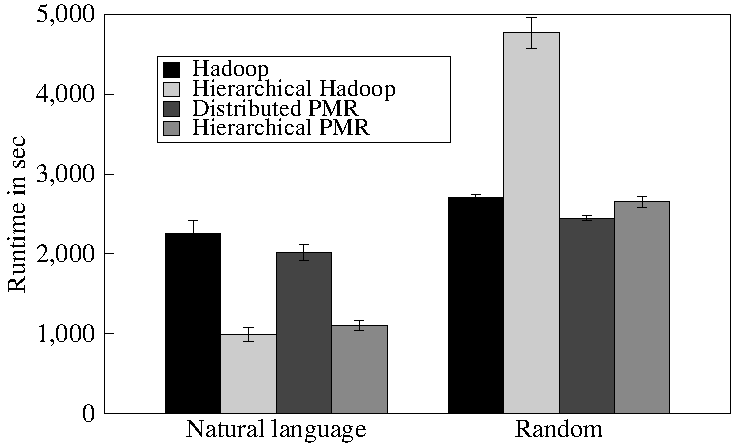
\includegraphics[width=0.47\textwidth]{figures/allmrs_rands.pdf}
\caption{Word Count on 16\,GB Data Using Hadoop, Hierarchical Hadoop, Distributed PMR  and Hierarchical PMR\upp} 	
\label{fig:allmrs_rands}
\end{figure}		


\subsubsection{Genome Sequencing}

\begin{figure}[ht]
	\centering
		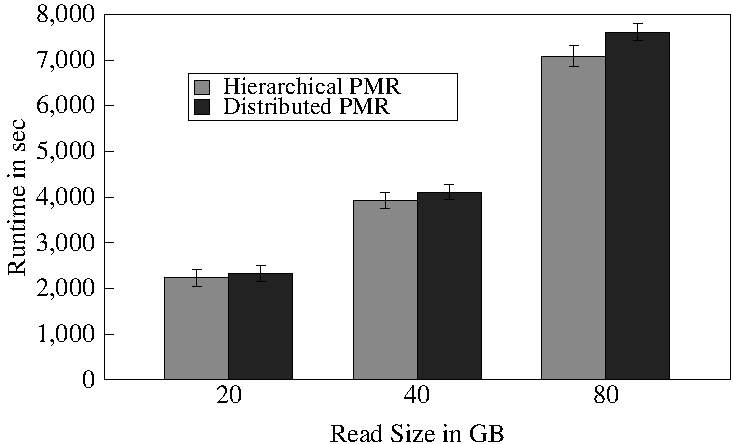
\includegraphics[width=0.47\textwidth]{figures/gs_hihmr_dpmr.pdf}
\caption{GS/PMR Using Hierarchical and Distributed PMR\upp\upp\upp} 	
\label{fig:gs_hihmr_dpmr}
\end{figure}		

For the genome sequencing application, we utilize India and Hotel, a total of 32
nodes and different input data size between 20 and 80\,GB.
Figure~\ref{fig:gs_hihmr_dpmr} shows the results. In both scenarios the runtime
increases with the input data size. For the distributed PMR, a significant part
of the performance is determined by the movement of the intermediate data --
71\,GB for the 80\,GB problem set (see table~\ref{tab:data-volumes}). In the
hierarchical PMR scenario, the main overhead arises from the additional
MapReduce run. For GS/PMR the hierarchical configuration shows a slight
advantage over the distributed setup since the amount of data that needs to be
transferred is significant less: half of the output, i.\,e.\ 8.5\,GB,
respectively, of the intermediate data, i.\,e.\ 36\,GB. However, a great amount 
of the time saving is absorbed by the overhead of the additional MapReduce run 
in the hierarchical case.

% Analysis
Running MapReduce on distributed data is not a trivial task -- the overall
performance is determined by many factors, e.\,g.\ the application's
characteristics, current machine and network loads, etc. Different MapReduce
configurations, such as the distributed and hierarchical configuration, can
address certain application characteristics. For example, depending on the
volume of the intermediate and output data, a distributed or hierarchical
configuration may show a better performance. In applications with a smaller
volume of output than intermediate data, such as GS and Word Count on natural
languages, a hierarchical MapReduce is a good choice since it involves less data
movement. PMR provides the flexibility to deploy MapReduce workloads in
different configurations optimizing the performance with respect to the
characteristics of different applications. Hadoop, in contrast, is very
inflexible in supporting different kind of MapReduce configurations. In our case
e.\,g.\ we were not able to run Hadoop across more than two machines on
FutureGrid due to firewall issues.


\subsubsection{Extensibility and Parallelism}
The extensibility of PMR is demonstrated with two aligners -- BWA and
Bowtie.  One of the important reasons why multiple aligners are needed
is because of the difficulty of validation of an aligner used\cite{mapping-survey}.  It is
well studied that each aligner implements different strategies to deal
with the requirement of computational loads, memory usage, and
sensitivity associated with decision on algorithms and computational
implementations of indexing, search, and match
tasks.

Indeed, the decision of which aligner affects not only alignment
results but also investigate downstream analysis that aim to study
genome variation, transcriptome analysis, and DAN-protein
interactions. Therefore, it is not an overstatement to emphasize the
importance of supporting multiple tools as well as providing an
effective means for implementing such tools within a reasonably short
development period for infrastructure of NGS data.

Fig.~\ref{fig:tool_comp}, evaluates the performance of read alignment
in the map phase of both Hadoop and PMR based applications for Bowtie
and BWA aligners. Hadoop implementations - Crossbow uses Bowtie
aligner and Seqal uses BWA aligner.  Custom python wrappers to Bowtie
and BWA aligner are developed to execute alignment in the map phase of
PMR. In the evaluation, both Hadoop based implementations face the
problem of non-optimal configuration of Hadoop, i.e usage of shared
file system for HDFS, where as both local and distributed PMR perform
better than Hadoop map phase for both aligners. The PMR is extensible
and can support multiple NGS analytic tools.

Extending PMR to support new NGS analytic tools involve development of
simple map and reduce wrapper scripts to the tools. The wrapper
scripts could be developed in any language.  To some extent, Hadoop streaming supports
this types of extensibility but still requires complexity of managing
computational resources to maintain Hadoop cluster.  PMR liberates the
user from the complex task of maintaining and acquiring computational
resources and executing map and reduce tasks on them.


\begin{figure} 
 \centering
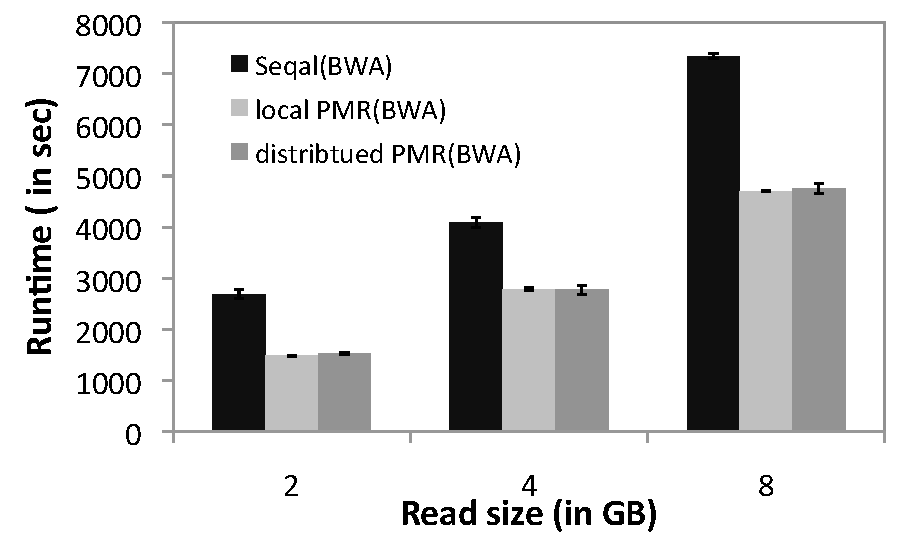
\includegraphics[scale=0.54]{figures/seqal_lpmr_dpmr.pdf}
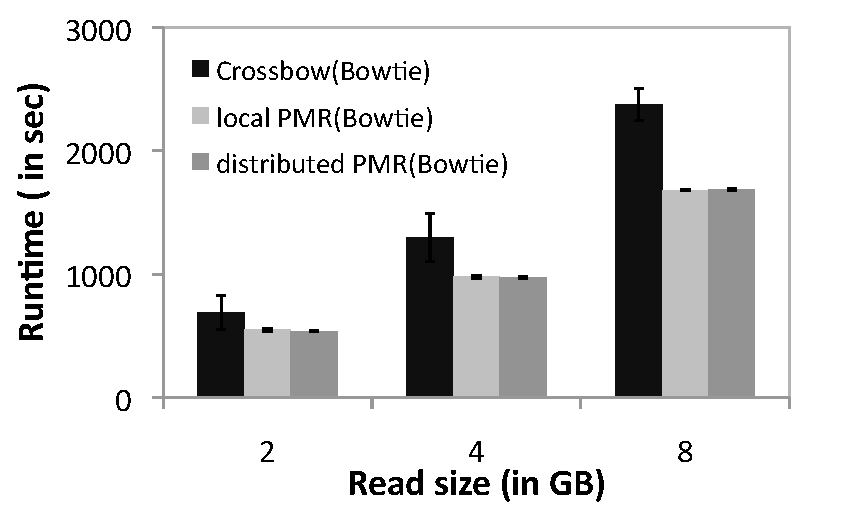
\includegraphics[scale=0.59]{figures/cb_lpmr_dpmr.pdf}
\caption{\small  Comparison of runtimes for the map phase. The map phase of Seqal, local-PMR(BWA), distributed-PMR(BWA), local-PMR(Bowtie), distributed-PMR(Bowtie), and Crossbow(Bowtie) are compared.  The aligner used for each case is indicated in a parenthesis.  For this experiment, the number of nodes, $N_{node}$ is 4, the number of Workers, $N_W$ is 8, and the number of reads in each chunk is 292,763.  For the distributed-PMR, two machines of FutureGrid, Sierra and Hotel were used, whereas Sierra was used for other cases.}
  \label{fig:tool_comp} 
\end{figure}


PMR supports multiple levels of parallelisms -- thread, task and
multiple-cores, and enables the flexible configurations of codes. For
example, BWA and Bowtie can be invoked to use varying number of
threads (fine-grained parallelism).  In Fig. \ref{fig:multi-parallel},
we showed how such options could affect the performance.  Even
though it is feasible for other tools such as Seqal or Crossbow to
handle such options, the PMR approach of separating the runtime
environment (Pilot) from the code invocation in the map and reduce
phases, provides the capability of utilizing the fine-grained
parallelism along with the coarse grain parallelism provided by
MapReduce. The fine grain parallelism provided by Pilot-Job framework is 
demonstrated in replica exchange implementation \cite{repex_ptrsa}.


\begin{figure} 
 \centering
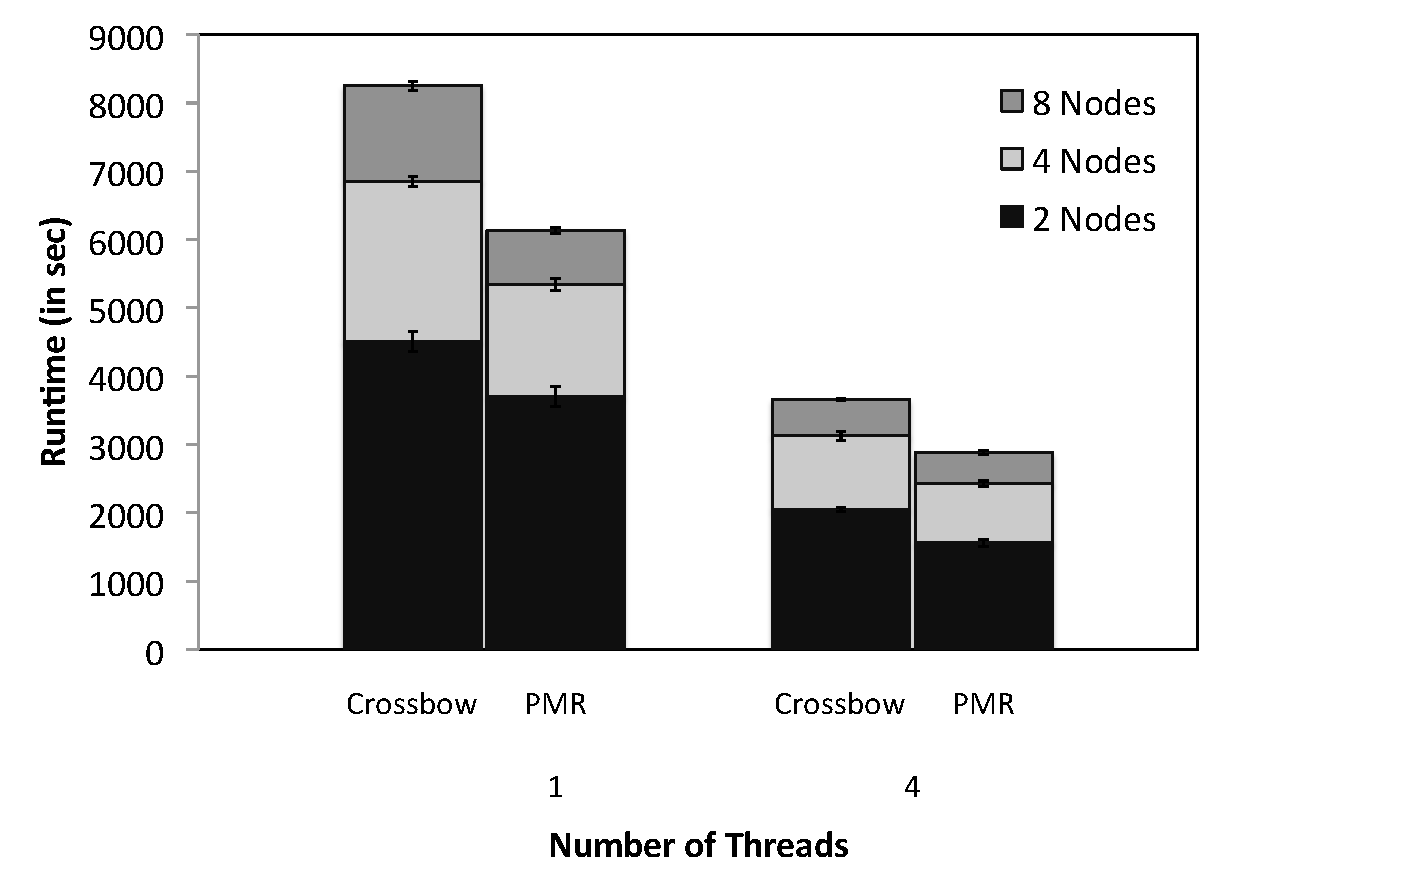
\includegraphics[scale=0.42]{figures/fig6_bw2.pdf}
\caption{\small The map phase runtimes of PMR(Bowtie) and Crossbow(Bowtie) are compared, by varying number of threads for each map task.  Number of workers/Node = 2 and input data size is 8 GB. The maximum number of cores assigned to a worker is 4, so we used 4 threads to achieve maximum fine-grain parallelism}
  \label{fig:multi-parallel} 
\end{figure}


One of the advantages of PMR is it doesn't impose any restriction on
number of compute nodes that can be assigned to a particular map or
reduce task. This leads to a natural and native support for MPI-based
NGS tools. For example,  NovoalignMPI~\cite{novo-align} is a message
passing version of Novoalign, with claims of a more accurate aligner,
allows a single alignment process to use multiple compute nodes. The
MPI versions of Novoalign are more beneficial when large computing
infrastructures are available.  Hadoop doesn't provide flexibility to
assign multiple compute nodes to a single compute task, thus leading
to an impedance mismatch between Hadoop MR and MPI based NGS analytic
tools.

%%%%%%%%%%%%%%%%%%%%%%%%%%%%%%%%%%%%%%%%
%New Chapter
%%%%%%%%%%%%%%%%%%%%%%%%%%%%%%%%%%%%%%%%
\chapter{Evaluation of BigJob on XSEDE and LONI}
\label{chap:pilot-lasigma}

%%%%%%%%%%%%%%%%%%%%%%%%%%%%%%%%%%%%%%%%
%New Chapter
%%%%%%%%%%%%%%%%%%%%%%%%%%%%%%%%%%%%%%%%

\chapter{Conclusions and Future Work}
\label{chap:conclusions}

\pilotmapreduce provides a flexible runtime environment for MapReduce
applications on general-purpose distributed infrastructures, such as XSEDE and
FutureGrid. It brings the advantages of the Pilot abstraction to MapReduce, and
enables utilization of federated and heterogeneous compute and data resources.
In contrast to Hadoop, no previous cluster setup, which includes running several
Hadoop/HDFS daemons, is required. Pilot-MapReduce provides a extensible runtime
environment, which allows the flexible usage of sorting in the shuffle, more
fine-grained control of data localities and transfer, as well as support for
different MapReduce topologies. Using these capabilities, applications with
different characteristics, e.\,g.\ compute/IO and data aggregation ratios, can
be efficiently supported. 

Pilot abstractions and the BigJob and BigData implementation
proofed to be a powerful tool for developing PMR. Using fine-granular affinity
specifications for compute/data units and resources, the runtime is able to
optimize compute and data placement as well as transfers. These capabilities are
essential for PMR especially when dealing with large amounts of distributed
data; to achieve an optimal performance in this case the application must be
able to reason and trade-off properties, such as data/compute localities and 
data transfers to achieve an optimal performance.

Future work in this research  may extend the capabilities of PMR and BigData to support use
cases, such as data streaming, data caching as well as different data/compute
scheduling heuristics. Further, explore scenarios and applications with
dynamic data and execution. An obvious and trivial extension will be to
implement Iterative MapReduce using PMR. A clear advantage will be to obviate
the need to distinguish between static and dynamic data, for PMR will be able to
treat both symmetrically.
\upp

%%%%%%%%%%%%%%%%%%%%%%%%%%%%%%%%%%%%%%%%
%%%%%%%%%%%%%%%%%%%%%%%%%%%%%%%%%%%%%%%%
\normalsize
\bibliographystyle{alpha}
\bibliographystyle{unsrt}
\bibliography{compbio,saga}
%%%%%%%%%%%%%%%%%%%%%%%%%%%%%%%%%%%%%%%%%%%%%%%%%%%%%%%%%%%%%%%%%%%%%%%%%%%%

\chapter*{Vita}
Pradeep Kumar Mantha is a computer science graduate student in the Louisiana State University. 
His interests lie in the bio-informatics, high-performance grid and supercomputing fields. 
He previously received a bachelor's degree from Jawaharlal Nehru and Technological University, Hyderabad, India.
\addcontentsline{toc}{chapter}{Vita}


\end{document}
